\section{Where to Adopt Personalization} \label{sec:where}

\subsection{Pre-retrieval} \label{sec:Pre-retrieval}

\subsubsection{\textbf{Definition}} Pre-retrieval is a crucial step in information retrieval systems, where the original user query is enhanced or modified before the retrieval process to improve the relevance and quality of the search results, as shown in Figure~\ref{fig:pre_rag}. This process often incorporates additional contextual or personalized information to better align the query with the user's intent. The process can be formalized as follows:
\begin{equation}
    q^{*} = \mathcal{Q}\left(q,p\right)
\end{equation}
where $p$ and $q$ denote the personalized information and original query, and $q^{*}$ is the optimized query after query reformulation.

\begin{figure}[t]
    \centering
    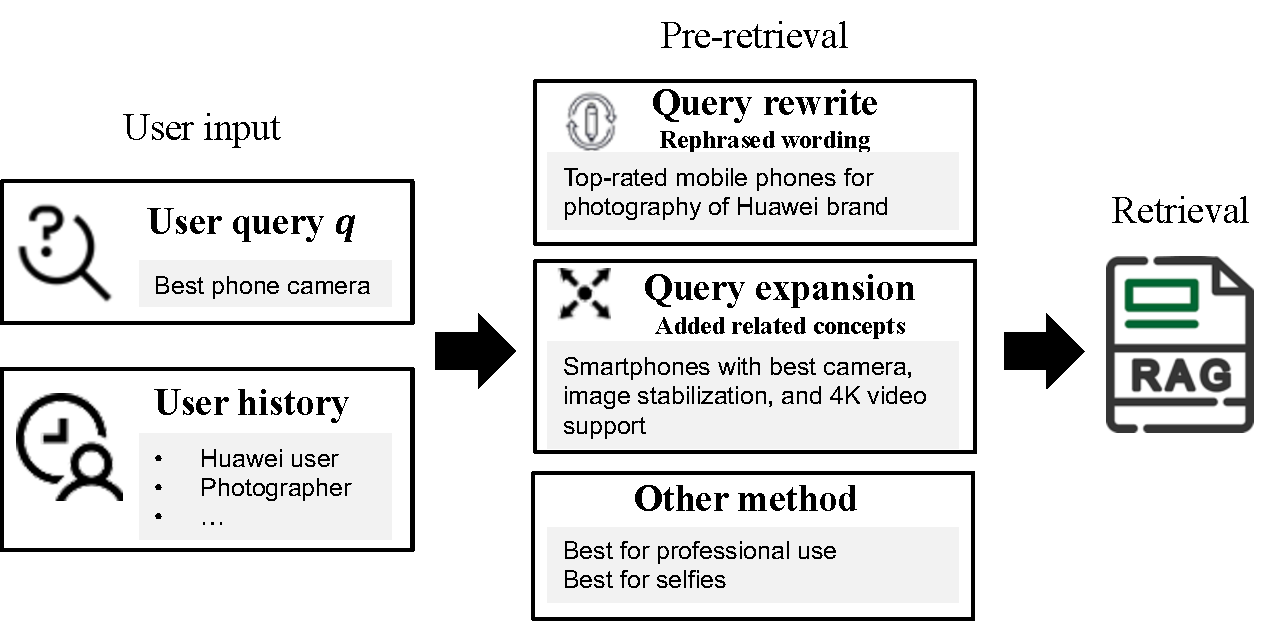
\includegraphics[width=1\linewidth]{figures/pre_rag.pdf}
    \caption{Overview of the personalized pre-retrieval stage.}
    \label{fig:pre_rag}
\end{figure}

\subsubsection{\textbf{Query Rewriting}}
Query rewriting in RAG at the pre-retrieval stage refers to the process of reformulating user queries to enhance retrieval effectiveness by improving relevance, disambiguating intent, or incorporating contextual information before retrieving documents from an external knowledge source.
The literature on personalized query rewriting can be broadly classified into two primary categories: (1) Direct Personalized Query Rewriting and (2) Auxiliary Personalized Query Rewriting.

\paragraph{\textbf{\textit{{(1). Direct Personalized Query Rewriting.}}}}

The first category focuses on personalized query rewriting by using direct models. 
For example, \citet{cho2021personalized} 
presents a personalized search-based query rewrite system for conversational AI that addresses user-specific semantic and phonetic errors. 
\citet{nguyen2025rl} apply reinforcement learning techniques to improve query rewriting in online e-commerce systems, leveraging distilled LLMs for personalized performance. 
CLE-QR~\cite{li2022query} explores query rewriting in Taobao's search engine to enhance user satisfaction through customized query adaptation. 
CGF~\cite{hao2022cgf} introduces a constrained generation framework that allows for more flexible and personalized query rewriting in conversational AI. 
\citet{li2024learning} investigate learning methods to rewrite prompts for personalized text generation, improving the relevance and engagement of AI-generated content. 
Additionally, PEARL~\cite{mysore2023pearl} discusses personalizing large language model-based writing assistants through the integration of generation-calibrated retrievers, enhancing AI-generated content.

\paragraph{\textbf{\textit{{(2). Auxiliary Personalized Query Rewriting.}}}} The second category emphasizes personalized query rewriting by using auxiliary mechanisms, such as retrieval, reasoning strategies, and external memory. 
\citet{zhou2022least} propose a least-to-most prompting strategy that aids in complex reasoning within LLMs, which can be adapted for personalized text generation.
ERAGent~\cite{shi2024eragent} enhance retrieval-augmented LLMs to improve personalization, efficiency, and accuracy, indirectly supporting personalized query rewriting for content generation. 
CoPS~\cite{zhou2024cognitive} integrate LLMs with memory mechanisms to create more personalized search experiences, which also influences content generation through better query understanding.
Further,  Agent4Ranking~\cite{li2023agent4ranking} employs multi-agent LLMs to perform semantic robust ranking, including personalized query rewriting to improve search rankings. 
FIG~\cite{chen2023graph} combine graph-based methods with LLMs to query rewrite, improving personalized content generation and conversational interactions. 
Lastly, BASES~\cite{ren2024bases} employ LLM-based agents to simulate large-scale web search user interactions, contributing to the development of personalized query rewriting strategies for content generation.


\subsubsection{\textbf{Query Expansion}}
Query expansion enhances retrieval systems by expanding a user’s original query with additional terms, synonyms, or refined structure to better capture intent. 
% \yc{the description here should be distinguished from that of query rewriting.} 
This improves the relevance and scope of retrieved documents. Recent advancements in LLMs have reinvigorated this field~\cite{wang2023query2doc,jagerman2023query,jia2024mill}, leveraging their comprehension and generation abilities to expand queries using encoded knowledge or external retrieval, with notable success. Personalized query expansion, a subset, incorporates user-specific data to tailor results, boosting performance and customizing the search experience.


\paragraph{\textbf{\textit{{(1). Tagging-based Query Expansion.}}}}

By 2009, studies began incorporating tagging information to enhance personalized query expansion. For instance, Gossple~\cite{bertier2009toward} introduced the TagMap and TagRank algorithms, which dynamically selected tags from personalized networks constructed using the cosine similarity of user-item tag distances, improving recall performance. Similarly,~\citet{biancalana2009social} recorded user queries and visited URLs, leveraging social bookmarking to extract relevant tags and build a personalized three-dimensional co-occurrence matrix. Based on this, multiple semantically categorized expanded queries were generated to better reflect user interests. Further advancements include SoQuES~\cite{bouadjenek2011personalized}, which integrated tag semantic similarity with social proximity, and a graph-based approach~\cite{zhou2012improving} that utilized Tag-Topic models and pseudo-relevance feedback for term weighting, tailoring the expansion process to individual user preferences.


\paragraph{\textbf{\textit{{(2). Else.}}}}
Apart from tagging-based techniques, early research on Personalized Query Expansion primarily focused on modeling user personalization based on search history~\cite{lin2006personalized}, social networks, or preferences derived from friendship networks~\cite{bender2008exploiting}. The Axiomatic PQEC framework~\cite{mulhem2016axiomatic} formalized expansion rules using both local (user behavior-driven) and social (network-driven) strategies. In 2017, WE-LM~\cite{wu2017personalized} advanced this paradigm by modeling multi-relational networks with word embeddings across tag-word relationships, refining associations through affinity graphs. Later, PSQE~\cite{bouadjenek2019personalized} further improved tagging-based methods using utf-iuf user profiling, integrating a tag similarity graph with user profiles in the online phase to compute expansion terms relevant to user interests in real-time, achieving dynamic personalized expansion. In addition, PQEWC~\cite{bassani2023personalized} leveraged clustering and contextual word embeddings to optimize query expansions dynamically.

\subsubsection{\textbf{Others}}

% \yc{Directly Besides is ok, rm subsection labels.}
Besides query rewriting and query expansion, other personalized query-related research focuses on areas like query disambiguation and query auto-completion~\cite{song2024survey}. Bobo~\cite{gao2010utilizing} allows users to input contextual terms reflecting their domain knowledge. In 2019, a method~\cite{kannadasan2019personalized} applied fastText embeddings from recent queries to rank candidates. In addition, PSQE~\cite{baumann2024psqe} employed synthetic user profiles from Wikipedia and word2vec embeddings for query disambiguation.

\subsubsection{\textbf{Discussion}}
While both query rewriting and query expansion aim to align user input with system understanding to enhance retrieval quality, their roles in personalization differ in fundamental ways.Understanding the distinct operational characteristics and application scenarios of each technique is essential for designing effective personalized retrieval systems. The key takeaways are listed as follows: 
\begin{itemize}[leftmargin=*] 
    \item Query rewriting is most beneficial when the original query is \textbf{ambiguous}, underspecified, or misaligned with retrieval intents, particularly in conversational or multi-turn settings. 
    \item Query expansion is most effective when the original query is \textbf{relevant} but incomplete — i.e., when it needs to be semantically broadened to cover additional relevant concepts.
\end{itemize}

